\chapter{Cinematica dei Robot}

\paragraph{}
In questo capitolo esploriamo la cinematica dei manipolatori robotici, i metodi per la rappresentazione dell'orientazione possono essere di due tipi: ridondanti e minimi.

\paragraph{}
Esempi di rappresentazioni minime: 
\begin{itemize}
\item angoli di Eulero ZYZ
\item angoli roll, pitch, yaw (rollio, beccheggio e imbardata)
\end{itemize}

\paragraph{}
Esempi di rappresentazioni ridondanti:
\begin{itemize}
	\item matrici di rotazione (9 numeri)
	\item quaternione unitario
\end{itemize}

\paragraph{}
Le rappresentazioni ridondanti si usano perchè evitano le singolarità algebriche, inevitabili usando le rappresentazioni minime.

\paragraph{}
Prima di iniziare, poniamo attenzione alla notazione: con $\underline{Q}$ indichiamo un vettore colonna di $\mathbb{R}^{n}$ e con una lettera maiuscola, come $A$ indichiamo una matrice.

\section{Matrici di Rotazione}

\paragraph{}
Scegliamo due terne cartesiane ortogonali $\langle0\rangle$, $\langle1\rangle$ ad origini distinte.\\

%due SdR, uno inerziale
\begin{tikzpicture} [y ={(1 cm ,0 cm )}, x ={( -0.5 cm , -0.5 cm )}, z ={(0 cm ,1 cm )}]
	\coordinate (0) at (0,0,0);
	\draw[->] (0)--(2,0,0) node [left] {$x_{0}$};
	\draw[->] (0)--(0,2,0) node [right] {$y_{0}$};
	\draw[->] (0)--(0,0,2) node [above] {$z_{0}$};
	\node[anchor = north] (0) at (0) {$O_{0}$};

	\coordinate (O1) at (0,6,0);
	\draw[->] (O1)--(2,6,0) node [left] {$x_{1}$};
	\draw[->] (O1)--(0,8,1) node [right] {$y_{1}$};
	\draw[->] (O1)--(0,5,2) node [above] {$z_{1}$};
	\node[anchor = north] (O1) at (O1) {$O_{1}$};
\end{tikzpicture}

\paragraph{}
Possiamo considerare $O_{0}$ e $O_{1}$ coincidenti, senza perdere di generalità. \\
Identifichiamo $\vec{i_{0}}$, $\vec{j_{0}}$, $\vec{k_{0}}$, $\vec{i_{1}}$, $\vec{j_{1}}$, $\vec{k_{1}}$ come i versori delle due terne. 
\paragraph{}
Adesso definiamo $\underline{^0i_{0}} \in \mathbb{R}^{3}$ come il vettore contenente le componenti di $\vec{i_{0}}$ in terna $\langle0\rangle$. Quindi, otteniamo:

\[\underline{^0i_{0}} = \begin{bmatrix}1\\0\\0\end{bmatrix}\]e il vettore $\underline{^0i_{1}}$ esprimibile come:
$\underline{^0i_{1}} = i_{1x}\cdot\underline{i} + i_{1y}\cdot\underline{j} + i_{1z}\cdot\underline{k}$

Nella terna $\langle0\rangle$ vale: $\underline{^0i_{0}} = \underline{i}, \, \underline{^0j_{0}} = \underline{j},\, \underline{^0k_{0}} = \underline{k}$ per evitare l'abuso di notazione.

\paragraph{}
Esprimendo i versori della terna $\langle1\rangle$ in terna $\langle0\rangle$, otteniamo:\\
\begin{equation}
	\begin{cases}
		\underline{^0i_{1}}=i_{1x}\cdot\underline{i} + i_{1y}\cdot\underline{j} + i_{1z}\cdot\underline{k}\\
		\underline{^0j_{1}}=j_{1x}\cdot\underline{i} + j_{1y}\cdot\underline{j} + j_{1z}\cdot\underline{k}\\
		\underline{^0k_{1}}=k_{1x}\cdot\underline{i} + k_{1y}\cdot\underline{j} + k_{1z}\cdot\underline{k}\\
	\end{cases}
\end{equation}
possiamo organizzare i 9 numeri in una matrice $3x3$ che battezziamo \emph{Matrice di Rotazione}, detta anche matrice dei coseni direttori:

%matrice di Rotazione
\begin{equation}
	R_{1}^{0} = 
	\begin{bmatrix}
		i_{1x} & j_{1x} & k_{1x} \\
		i_{1y} & j_{1y} & k_{1y} \\
		i_{1z} & j_{1z} & k_{1z} \\
	\end{bmatrix}
	= 
	\begin{bmatrix}
		\:\underline{^0i_{1}} \quad \underline{^0j_{1}} \quad\underline{^0k_{1}}\:
	\end{bmatrix}
\end{equation}

\subsection{Codifica l'orientazione}
\paragraph{}
La prima utilità di $R_{1}^{0}$ è quella di codificare l'orientazione relativa di $\langle1\rangle$ rispetto a $\langle0\rangle$, attraverso i versori di $\langle1\rangle$ espressi in terna $\langle0\rangle$.

\subparagraph{Espressione di $R_{1}^{0}$ per rotazione attorno all'asse $z$}
\paragraph{}%SdR pg 3
\begin{figure}[ht]
	\begin{minipage}[b]{0.45\linewidth}
		\centering
		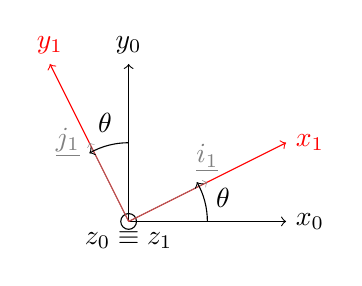
\begin{tikzpicture}[y ={(0 cm ,1 cm )}, x ={( 1 cm , 0 cm )}]
			\coordinate (O) at (0,0);
			\draw[->] (O)--(2,0) node [right] {$x_{0}$};
			\draw[->] (O)--(0,2) node [above] {$y_{0}$};
			\draw  (O) circle [ radius = 0.1 cm] node [below] {$z_{0}\equiv z_{1}$};
			\draw[->, color = red] (O)--(2,1) node [right] {$x_{1}$};
			\draw[help lines, ->] (O)--(1,0.5) node [above] {$\underline{i_{1}}$};
			\draw[->, color = red] (O)--(-1,2) node [above] {$y_{1}$};
			\draw[help lines, ->] (O)--(-0.5,1) node [left] {$\underline{j_{1}}$};
			\draw [->] (1,0) arc(0:30:1);
			\node at (1.2cm, 0.3cm) {$\theta$};
			\draw [->] (0,1) arc(90:120:1);
			\node [above] at (-0.3cm, 1cm) {$\theta$};
		\end{tikzpicture}
	\end{minipage}
	\begin{minipage}[b]{0.45\linewidth}
		\centering
		\begin{equation*}
			R_{1}^{0} = 
			\begin{bmatrix}
				\cos(\theta) & -\sin(\theta) & 0 \\
				\sin(\theta) & \cos(\theta) & 0 \\
				0 & 0 & 1 \\
			\end{bmatrix}
		\end{equation*}
	\end{minipage}
\end{figure}
\newpage %interruzione di pagina

\subparagraph{Espressione di $R_{1}^{0}$ per rotazione attorno all'asse $x$}
\paragraph{}%SdR pg 3
\begin{figure}[ht]
	\begin{minipage}[b]{0.45\linewidth}
		\centering
		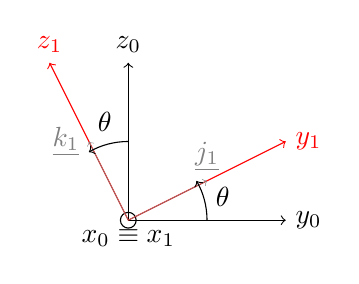
\begin{tikzpicture}[y ={(0 cm ,1 cm )}, x ={( 1 cm , 0 cm )}]
			\coordinate (O) at (0,0);
			\draw[->] (O)--(2,0) node [right] {$y_{0}$};
			\draw[->] (O)--(0,2) node [above] {$z_{0}$};
			\draw  (O) circle [ radius = 0.1 cm] node [below] {$x_{0}\equiv x_{1}$};
			\draw[->, color = red] (O)--(2,1) node [right] {$y_{1}$};
			\draw[help lines, ->] (O)--(1,0.5) node [above] {$\underline{j_{1}}$};
			\draw[->, color = red] (O)--(-1,2) node [above] {$z_{1}$};
			\draw[help lines, ->] (O)--(-0.5,1) node [left] {$\underline{k_{1}}$};
			\draw [->] (1,0) arc(0:30:1);
			\node at (1.2cm, 0.3cm) {$\theta$};
			\draw [->] (0,1) arc(90:120:1);
			\node [above] at (-0.3cm, 1cm) {$\theta$};
		\end{tikzpicture}
	\end{minipage}
	\begin{minipage}[b]{0.45\linewidth}
		\centering
		\begin{equation*}
			R_{1}^{0} = 
			\begin{bmatrix}
				1 & 0 & 0 \\
				0 & \cos(\theta) & -\sin(\theta) \\
				0 & \sin(\theta) & \cos(\theta) \\
			\end{bmatrix}
		\end{equation*}
	\end{minipage}
\end{figure}

\subparagraph{Espressione di $R_{1}^{0}$ per rotazione attorno all'asse $y$}
\paragraph{}%SdR pg 3
\begin{figure}[ht]
	\begin{minipage}[b]{0.45\linewidth}
		\centering
		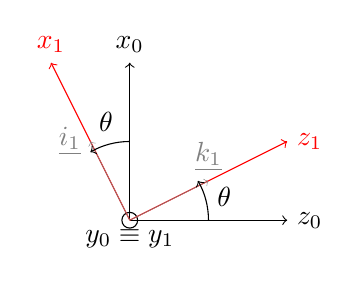
\begin{tikzpicture}[y ={(0 cm ,1 cm )}, x ={( 1 cm , 0 cm )}]
			\coordinate (O) at (0,0);
			\draw[->] (O)--(2,0) node [right] {$z_{0}$};
			\draw[->] (O)--(0,2) node [above] {$x_{0}$};
			\draw  (O) circle [ radius = 0.1 cm] node [below] {$y_{0}\equiv y_{1}$};
			\draw[->, color = red] (O)--(2,1) node [right] {$z_{1}$};
			\draw[help lines, ->] (O)--(1,0.5) node [above] {$\underline{k_{1}}$};
			\draw[->, color = red] (O)--(-1,2) node [above] {$x_{1}$};
			\draw[help lines, ->] (O)--(-0.5,1) node [left] {$\underline{i_{1}}$};
			\draw [->] (1,0) arc(0:30:1);
			\node at (1.2cm, 0.3cm) {$\theta$};
			\draw [->] (0,1) arc(90:120:1);
			\node [above] at (-0.3cm, 1cm) {$\theta$};
		\end{tikzpicture}
	\end{minipage}
	\begin{minipage}[b]{0.45\linewidth}
		\centering
		\begin{equation*}
			R_{1}^{0} = 
			\begin{bmatrix}
				\cos(\theta) & 0 & \sin(\theta) \\
				0 & 1 & 0 \\
				-\sin(\theta) & 0 & \cos(\theta) \\
			\end{bmatrix}
		\end{equation*}
	\end{minipage}
\end{figure}

\paragraph{}
Notiamo che in generale il $\det(R_{1}^{0}) = 1 $, quindi $R_{1}^{0}$ è invertibile, ma solo se parliamo di rotazione sinistrorsa (o levogira). Infatti, nel caso la matrice $R_{1}^{0}$ sia destrorsa allora si ha che $\det(R_{1}^{0}) = -1 $.

\subsection{Cambio di coordinate di un punto dello spazio}

\paragraph{}
Usiamo la matrice $R$ per cambiare le coordinate di un punto dello spazio tra terne ad origine comune. 


\paragraph{}
\begin{center}
	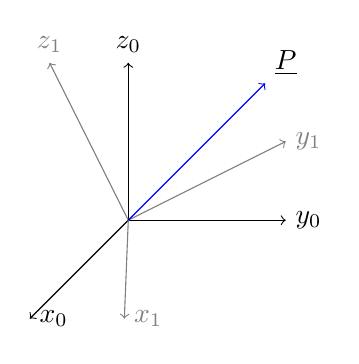
\begin{tikzpicture}[y ={(1cm, 0cm)}, x ={(-0.5cm, -0.5cm)}, z ={(0 cm, 1 cm)}]
		\coordinate (O) at (0,0,0);
		\draw[->] (O) -- (0,2,0) node [right] {$y_{0}$};
		\draw[->] (O) -- (0,0,2) node [above] {$z_{0}$};
		\draw[->] (O) -- (2.5,0,0) node [right] {$x_{0}$};

		\draw[->, gray] (O) -- (0,2,1) node [right] {$y_{1}$};
		\draw[->, gray] (O) -- (0,-1,2) node [above] {$z_{1}$};
		\draw[->, gray] (O) -- (2.5,1.2,0) node [right] {$x_{1}$};
	
		\node (P) at (0,2,2) {$\underline{P}$};
		\draw[->, blue] (O) -- (P);
	\end{tikzpicture}
\end{center}

$\vec{O_{o}P}$ possiamo esprimerlo in terna $\langle 0 \rangle$ oppure in terna $\langle 1 \rangle$. Ovvero: 

$\underline{^{0}P} = 
	\begin{bmatrix}
		p_{0x} & p_{0y} & p_{0z}
	\end{bmatrix}^{T}\quad$
e 
$\quad\underline{^{1}P} = 
	\begin{bmatrix}
		p_{1x} & p_{1y} & p_{1z}
	\end{bmatrix}^{T}$
	
\paragraph{}
Otteniamo: $p_{0x}\:\underline{i}+p_{0y}\:\underline{j}+p_{0z}\:\underline{k} = p_{1x}\:\underline{^0i_{1}}+p_{1y}\:\underline{^0j_{1}}+p_{1z}\:\underline{^0k_{1}}$ e ho quindi espresso $\underline{^0P}$ in due modi e allora posso riscrivere il vettore come segue: 

\begin{equation}
	\underline{^0P}=
	\begin{bmatrix}
		\;\underline{^0i_{1}} & \underline{^0j_{1}} & \underline{^0k_{1}}\;
	\end{bmatrix}
	\begin{bmatrix}
		p_{1x} \\
		p_{1y} \\
		p_{1z}
	\end{bmatrix}
	= R_{1}^{0} \: \underline{^1P}	
\end{equation}
Questa relazione non vale solo per i vettori posizione, ma anche per velocità, velocità angolari, forze, ecc...

\subsection{Proprietà di $R$}
\begin{itemize}
	\item $\det(R) = \vert R \vert = 1$
	\item $R^{\,-1} = R^{T}$
	\item $R^{T}R = I$
\end{itemize}
Quest'ultima proprietà si dimostra ponendo, 
\begin{equation*}
	R_1^0 =
	\begin{bmatrix}
		\:\underline{^0i_1} & \underline{^0j_1} & \underline{^0k_1}\:
	\end{bmatrix}
	= R
\end{equation*} e facendo il prodotto con la sua trasposta, ottengo:
\begin{equation*}
	R^{T} \cdot R =
	\begin{bmatrix}
		\:\underline{^0i_1}\: \\
		\:\underline{^0j_1}\: \\
		\:\underline{^0k_1} \:
	\end{bmatrix}
	\cdot
	\begin{bmatrix}
		\: \underline{^0i_1} & \underline{^0j_1} & \underline{^0k_1} \:
	\end{bmatrix}
	= 
	\begin{bmatrix}
		1 & 0 & 0 \\
		0 & 1 & 0 \\
		0 & 0 & 1 
	\end{bmatrix}
	= I_{3x3}
\end{equation*}

\subsection{Derivata temporale di $R$}
\paragraph{}
Per due terne $\langle 0 \rangle$, $\langle 1 \rangle$ in moto relativo tra loro, vale $R = R(t)$, senza perdere di generalità, supponiamo $O_0 = O_1$ e scegliamo un punto $\underline{P}$ fisso in terna $\langle 1 \rangle$. Deriviamo quindi $\underline{^0P} = R_{1}^{0} \cdot \underline{^1P}$ e otteniamo:

\begin{equation}
	\dfrac{d}{dt} \; (^0\underline{P}) = \underline{^0\dot{P}} = \dot{R_{1}^{0}}\; ^1\underline{P} + R_{1}^{0} \; ^1\underline{\dot{P}} = \dot{R_{1}^{0}}\; ^1\underline{P}
\end{equation}
Utilizzando la formula fondamentale dei moti rigidi 
\begin{equation}
	\underline{\dot{P}} = \underline{\dot{O_{1}}} + \underline{^0\omega_{1}} \times R_{1}^{0}\: \underline{^1P} = \underline{\dot{O_{1}}} + \underline{^0\omega_{1}} \times \: \underline{^0P}
\end{equation}
Uguagliando la (1.4) e la (1.5) otteniamo: 
\begin{equation}
	\dot{R_{1}^{0}}\;\underline{^1P} = \underline{^0\omega_{1}} \times ( R_{1}^{0} \; \underline{^1P}) = S(^0\omega_{1}) \; R_{1}^{0} \; \underline{^1P}
\end{equation} 
Isolando la matrice di rotazione otteniamo le \emph{Formule di Poisson} "condensate" in una sola matriciale:
\begin{equation}
	\dot{R_{1}^{0}} = S(^0\omega_{1}) \; R_{1}^{0} 
\end{equation}

\subparagraph{Notiamo la funzione $S(\cdot)$:}
Il prodotto vettoriale $ \underline{a} \times \underline{b} $ viene espresso mediante l'uso della funzione (\emph{formalismo matriciale}):
\begin{equation*}
	S(\underline{a}) = 
	\begin{bmatrix}
		0 & -a_z & a_y \\
		a_z & 0 & -a_x \\
		-a_y & a_x & 0
	\end{bmatrix}
\end{equation*}
e quindi risulta: $\underline{a} \times \underline{b} = S(\underline{a}) \; \underline{b}$ e inoltre notiamo la proprietà $S^T(\cdot) = - S(\cdot)$.

\section{Rotazioni nello spazio}
\paragraph{}
Consideriamo di \emph{ruotare un vettore nello spazio}, cioè andiamo a \emph{premoltiplicare} una certa matrice di rotazione $R$ per un vettore $\underline{v}$ dato. Noi abbiamo:
\begin{equation*}
	\underline{v} = \vert\underline{v}\vert \; 
	\begin{bmatrix}
		\cos(\alpha) \\
		\sin(\alpha) \\
		0
	\end{bmatrix}	
	\qquad
	R =
	\begin{bmatrix}
		\cos(\beta) & -\sin(\beta) & 0 \\
		\sin(\beta) & \cos(\beta) & 0 \\
		0 & 0 & 1
	\end{bmatrix}
\end{equation*}
e otteniamo $\underline{w}=R\,\underline{v}$, vediamo come è fatto $\underline{w}$:
\begin{align*}
	\underline{w} = 
	\begin{bmatrix}
		w_x \\
		w_y \\
		w_z
	\end{bmatrix}
	=
	\begin{bmatrix}
		\cos(\beta) & -\sin(\beta) & 0 \\
		\sin(\beta) & \cos(\beta) & 0 \\
		0 & 0 & 1
	\end{bmatrix}
	\begin{bmatrix}
		\cos(\alpha) \\
		\sin(\alpha) \\
		0
	\end{bmatrix}
	\vert\underline{v}\vert = \\
	=
	\begin{bmatrix}
		\cos(\alpha)\cos(\beta) - \sin(\alpha)\sin(\beta) \\
		\cos(\alpha)\sin(\beta) - \cos(\alpha)\sin(\beta) \\
		0
	\end{bmatrix}
	\vert\underline{v}\vert = 
	\begin{bmatrix}
		\cos(\alpha + \beta) \\
		\sin(\alpha + \beta) \\
		0
	\end{bmatrix}
	\vert\underline{v}\vert
\end{align*}
quindi, $\forall\underline{v}$ e $\forall R$ \emph{allora} $\underline{w} = R \underline{v}$ è un vettore con lo stesso modulo di $\underline{v}$ ruotato nello spazio, di un certo angolo ed attorno ad un certo asse, \emph{codificati in $R$}.

\paragraph{}
Possiamo fare delle \emph{rotazioni successive} nello spazio, e abbiamo due possibilità: 
\begin{itemize}
	\item composizione di rotazioni specificate in \emph{terna corrente}
	\item composizione di rotazioni specificate in \emph{terna fissa}
\end{itemize}

\subsection{Rotazioni in terna corrente}
\paragraph{}
Supponiamo di avere tre terne $\langle0\rangle$, $\langle1\rangle$, $\langle2\rangle$ ad origine comune ed un punto $\underline{P}$.

\begin{equation*}
	\begin{cases}
		^0\underline{P} = R_1^0 \, ^1\underline{P} \\
		^1\underline{P} = R_2^1 \, ^2\underline{P} \\
		^0\underline{P} = R_2^0 \, ^2\underline{P}
	\end{cases}
	\Rightarrow
	\begin{cases}
		^0\underline{P} = R_1^0 \, R_2^1 \, ^2\underline{P} \\
		^0\underline{P} = R_2^0 \, ^2\underline{P}
	\end{cases}
	\Rightarrow
	R_2^0 = R_1^0 \, R_2^1
\end{equation*}

Si generalizza a $n+1$ terne:  
\begin{equation}
	R_n^0 = R_1^0 \, R_2^1 \, \cdots R_{n-1}^{n-2} \, R_{n}^{n-1}
\end{equation}

ottenendo la \emph{Matrice che mappa la terna $n$ nella terna $0$}.
\newpage

\subsection{Rotazioni in terna fissa}
\paragraph{}
Supponiamo di avere tre terne $\langle0\rangle$, $\langle1\rangle$, $\langle2\rangle$ ad origine comune e che la terna $\langle 0 \rangle$ sia fissa. Quindi, definiamo:
\begin{itemize}
	\item $R_1^0$ trasforma i versori principali della terna $\langle 0 \rangle$ (espressi in $\langle 0 \rangle$) nei versori principali della terna $\langle 1 \rangle$ espressi in $\langle 0 \rangle$.
	\item $^0R_2^1$ trasforma i versori principali della terna $\langle 1 \rangle$ nei versori principali della terna $\langle 2 \rangle$ entrambi \emph{espressi in terna $\langle 0 \rangle$}.
\end{itemize}

Con la notazione appena introdotta è facile verificare che $R_1^0 \equiv \,^0R_1^0$.
\paragraph{}
Applichiamo $^0R_2^1$ ai versori di $\langle1\rangle$, otteniamo:
\begin{equation*}
	\begin{cases}
		^0\underline{i_2} = ^0R_2^1 \, ^0\underline{i_1} \\
		^0\underline{j_2} = ^0R_2^1 \, ^0\underline{j_1} \\
		^0\underline{k_2} = ^0R_2^1 \, ^0\underline{k_1}
	\end{cases}
	\Leftrightarrow
	\begin{bmatrix}
		^0\underline{i_2} & ^0\underline{j_2} & ^0\underline{k_2}
	\end{bmatrix}
	= \,^0R_2^1 \,
	\begin{bmatrix}
		^0\underline{i_1} & ^0\underline{j_1} & ^0\underline{k_1}
	\end{bmatrix}
\end{equation*}  

ovvero:
\begin{equation*}
	^0R_2^0 = \,^0R_2^1 \, ^0R_1^0
\end{equation*}

E generalizzando otteniamo la \emph{regola di composizione di rotazioni in terna fissa}:
\begin{equation}
	^0R_n^0 = \,^0R_n^{n-1} \cdot \,^0R_{n-1}^{n-2} \,  \cdots \, ^0R_{2}^{1} \cdot \,^0R_{1}^{0}
\end{equation}
Vediamo come calcolare $^0R_2^1$:

\begin{equation}
	\begin{cases}
		R_2^0 = R_1^0\,R_2^1 \\
		R_2^0 = \,^0R_2^1\,R_1^0 
	\end{cases}
	\Rightarrow
	R_1^0\,R_2^1 = \,^0R_2^1\,R_1^0 \;
	\Rightarrow \;
	^0R_2^1 = R_1^0\,R_2^1\,(R_1^0)^T
\end{equation}

ho espresso le due composizioni e ho moltiplicato per $(R_1^0)^T$.

\subsubsection{Non commutatività delle rotazioni}
Il prodotto matriciale non è commutativo, così come \emph{non} lo sono le rotazioni, vediamo infatti un esempio in terna corrente:

\includegraphics[scale=0.35]{rotazioniNonCommutative.pdf}
\newpage

\section{Rappresentazione Asse - Angolo}
Si parte dal ricavare la $R$ corrispondente ad una rotazione di $\theta$ (arbitrario) attorno ad un asse identificato da un versore $\underline{r}$ (arbitrario). $\underline{r}$ è univocamente determinato da $\alpha$ e $\beta$ e poi vedremo il contrario.

\includegraphics[scale=0.35]{asseAngolo.pdf}
\captionof{figure}{Rotazione di un angolo intorno ad un asse}

\subsection{Ricavare $R$ partendo da asse e angolo}
Dato che non sappiamo scrivere di getto $R_{\underline{r}}(\theta)$, otteniamola come \emph{successione di rotazioni specificate in terna fissa}:
\begin{enumerate}
	\item Attorno all'asse $z$ di $- \alpha$
	\item Attorno all'asse $y$ di $- \beta$
	\item Attorno all'asse $z$ di $\theta$ ($\Rightarrow rotazione\;desiderata$)
	\item Attorno all'asse $y$ di $\beta$
	\item Attorno all'asse $z$ di $\alpha$
\end{enumerate}
Notiamo che i passi \emph{1 e 2} servono per allineare $\underline{r}$ corrente con $z$ (terna fissa) e stiamo specificando le rotazioni sempre in terna fissa, quindi la produttoria si fa dall'ultima alla prima:
\begin{equation}
	R_{\underline{r}}(\theta) = R_{z}(\alpha)\,R_{y}(\beta)\,R_{z}(\theta)\,R_{y}(-\beta)\,R_{z}(-\alpha) 
\end{equation}
$\cdots$ dopo un pò di lavoro algebrico, otteniamo:

\begin{equation*}
	R_{\underline{r}}(\theta) =
	\begin{bmatrix}
		r_x^2\,(1-C_{\theta})+C_{\theta} & r_x r_y\,(1-C_{\theta})-r_z\,S_{\theta} & r_x r_z\,(1-C_{\theta})+r_y\,S_{\theta} \\
		r_x r_y\,(1-C_{\theta})+r_z\,S_{\theta} & r_y^2\,(1-C_{\theta})+C_{\theta} & r_y r_z\,(1-C_{\theta})-r_x\,S_{\theta} \\
		r_x r_z\,(1-C_{\theta})-r_y\,S_{\theta} & r_y r_z\,(1-C_{\theta})+r_x\,S_{\theta} & r_z^2\,(1-C_{\theta})+C_{\theta} 
	\end{bmatrix}
\end{equation*}

con $C_{\theta} = \cos(\theta)$ e $S_{\theta} = \sin(\theta)$.

\subsection{Ricavare asse e angolo partendo da $R$}
Adesso vediamo come ricavare $r_x$, $r_y$, $r_z$ e $\theta$ data una matrice $R$ qualsiasi. Valutiamo la \emph{traccia di $R$}:
 
\begin{equation*}
	T_{r}(R)= r_{11} + r_{22} + r_{33} = 1 + 2\, \cos(\theta) \Rightarrow \theta = \pm \arccos\Bigl(\dfrac{r_{11} + r_{22} + r_{33} - 1}{2}\Bigr)
\end{equation*}
Otteniamo due rami di soluzione perchè una rotazione $\langle\underline{r}, \theta\rangle$ è identica, come risultato, ad una rotazione $\langle-\underline{r}, -\theta\rangle$.

\paragraph{}
Adesso calcoliamo $r_x, r_y, r_z$:

\subparagraph{• Se $\sin(\theta) \neq 0$}:
Sottraiamo $r_{12}$ a $r_{21}$ e facciamo analogamente con gli altri, otteniamo:
\begin{equation*}
	\begin{cases}
		r_{21}-r_{12} = 2 \, r_z \sin(\theta)\\
		r_{13}-r_{31} = 2 \, r_y \sin(\theta)\\
		r_{32}-r_{23} = 2 \, r_x \sin(\theta)
	\end{cases}
	\Rightarrow
	\begin{bmatrix}
		r_x \\
		r_y \\
		r_z 
	\end{bmatrix}
	= \dfrac{1}{2\,\sin(\theta)}
	\begin{bmatrix}
		r_{32}-r_{23} \\
		r_{13}-r_{31} \\
		r_{21}-r_{12}
	\end{bmatrix}
\end{equation*}

\subparagraph{• Se $\sin(\theta) = 0$}:
In questo caso particolare, possono accadere due situazioni,

\begin{enumerate}
	\item $\cos(\theta) = 1 \quad \Rightarrow \,\theta = 0$ (rotazione nulla) 
	\item $\cos(\theta) = -1 \quad \Rightarrow \,\theta = \pm \pi $ (caso più interessante)
\end{enumerate}

Nel secondo caso, la matrice diventa:
\begin{equation}
	R_{\underline{r}}(\pm \pi) = 
	\begin{bmatrix}
		2\,r_x^2 - 1 & 2\,r_x\,r_y & 2\,r_x\,r_z \\	
		2\,r_x\,r_y & 2\,r_y^2 - 1 & 2\,r_y\,r_z \\
		2\,r_x\,r_z & 2\,r_y\,r_z &  2\,r_z^2 - 1
	\end{bmatrix}	 
\end{equation}

quindi, 
\begin{equation}
	r_{11} = 2\,r_x^2 - 1 \quad \Rightarrow \quad r_x^2 = \dfrac{r_{11}+1}{2} \quad\Rightarrow \quad r_x = \pm \sqrt{\dfrac{r_{11}}{2}}
\end{equation}

a questo, dobbiamo valutare se $\vert r_x \vert > \varepsilon$ dove con $\varepsilon$ indichiamo una soglia numerica per discriminare il caso in cui $\sin(\theta) \neq 0$, otteniamo:
\begin{equation*}
	se\,\vert r_x \vert > \varepsilon \quad \Rightarrow \quad 
	\begin{cases}
		r_y = \dfrac{r_{12}}{2r_x} \\
		r_z =\dfrac{r_{13}}{2r_x}
	\end{cases}	
\end{equation*}

se la condizione non dovesse essere rispettata, provo a esplicitare $r_y$ o $r_z$ e fare il controllo su di loro.
\newpage

\begin{Esercizio}
	Consideriamo la pinza $\underline{n},\underline{s},\underline{a},$ ovvero \emph{Normal, Sliding, Approach}
	\includegraphics[scale=0.35]{pinzaNSA.pdf}\\
	e consideriamo la matrice:
	\begin{equation*}
		R = 
		\begin{bmatrix}
			n_x & 1 & a_x \\
			0 & s_y & a_y \\
			1 & s_z & a_z
		\end{bmatrix}
	\end{equation*}
	ci chiediamo quanto valgono i termini incogniti. Sfruttando le proprietà di $R$, possiamo dire che $n_x = s_y = s_z = 0$ perchè le colonne devono essere a norma unitaria.\\
	Sappiamo che $\underline{n} \times \underline{s} = \underline{a}$ e sfruttando la \emph{rappresentazione matriciale} del prodotto vettoriale, otteniamo:
	\begin{equation*}
		S(\underline{n})\cdot\underline{s} = 
		\begin{bmatrix}
			0 & -1 & 0 \\
			1 & 0 & 0 \\
			0 & 0 & 0 
		\end{bmatrix}
		\begin{bmatrix}
			1 \\
			0 \\
			0
		\end{bmatrix}
		= 
		\begin{bmatrix}
			0 \\
			1 \\
			0
		\end{bmatrix}
	\end{equation*}
	e otteniamo:
	\begin{equation*}
		R = 
		\begin{bmatrix}
			0 & 1 & 0 \\
			0 & 0 & 1 \\
			1 & 0 & 0 
		\end{bmatrix}
	\end{equation*}
\end{Esercizio}


\newpage
\section{Angoli di Eulero $ZYZ$}
\paragraph{}
Si tratta di una rappresentazione minima che utilizza tre angoli, si fissano due terne: 
\begin{itemize}
	\item terna $\langle0\rangle$ fissa
	\item terna $\langle1\rangle$ mobile rispetto a $\langle0\rangle$
\end{itemize}
Il concetto è che \emph{tre rotazioni successive} in terna corrente formano la \emph{rotazione complessiva}. 
\paragraph{}
Intersecando i piani $x_0y_0$ e $x_1y_1$ si ottiene una retta che chiamiamo \textbf{Linea dei Nodi}. Notiamo che questa linea non è univocamente determinata quando $\underline{k_0} = \pm \underline{k_1}$, ovvero, quando i piani sono paralleli. Inoltre, la linea dei nodi è $\perp$ sia a $z_0$ che a $z_1$.

\includegraphics[scale=0.35]{angoliEulero.pdf}
\captionof{figure}{Angoli di Eulero}

\subsubsection{Tre Rotazioni}
\begin{enumerate}
	\item Ruotiamo la terna $\langle0\rangle$ attorno a $z_0$ di un angolo $\varphi$ fino a che $y$ della terna corrente non si allinea con la \emph{linea dei nodi}. Chiamiamo la \emph{terna corrente} $O_{x'y'z'}$ con $z' \equiv z_0$.
	\item Imponiamo, alla terna corrente $O_{x'y'z'}$, una rotazione attorno a $y'$ (\emph{linea dei nodi} $\perp \underline{k_0} \perp \underline{k_1}$ ) di un angolo $\theta$ fino a che l'asse $z$ della \emph{terna corrente} non si allinea con $z_1$. Chiamiamo questa terna $O_{x"y"z"}$ con $y" \equiv y'$ e $z" = z_1$. A questo punto, $z$ è nella sua orientazione, $y" \equiv y'$ è la \emph{linea dei nodi} e $x"y"$ è ruotato di un certo angolo $\psi$ rispetto a $x_1y_1$.
	\item Imponiamo una rotazione $\psi$ attorno a $\underline{k"} \equiv \underline{k_1}$ fino a che $x$ e $y$ della terna corrente non si allineano con $x_1$ e $y_1$.
\end{enumerate}
Otteniamo la composizione in terna corrente seguente:
\begin{equation}
	R_{zyz} = R_z(\varphi)R_{y'}(\theta)R_{z"}(\psi)
\end{equation}

con $z \equiv z_0$, $y' = $\emph{ linea dei nodi} e $z" \equiv z_1$. 

\begin{center}
\includegraphics[scale=0.35]{rotazioniEulero.pdf}
\captionof{figure}{Rotazioni di Eulero: a)$R_z(\varphi)$ b)$R_{y'}(\theta)$ c)$R_{z_1}(\psi)$}
\end{center}


\paragraph{}
Scriviamo la matrice complessiva $R_{zyz}$:

\begin{equation*}
	R_{zyz} = R_z(\varphi)R_{y'}(\theta)R_{z"}(\psi) =
	\begin{bmatrix}
		C_{\varphi} & -S_{\varphi} & 0 \\
		S_{\varphi} & C_{\varphi} & 0 \\
		0 & 0 & 1
	\end{bmatrix}
	\cdot
	\begin{bmatrix}
		C_{\theta} & 0 & S_{\theta} \\
		0 & 1 & 0 \\
		-S_{\theta} & 0 & C_{\theta}
	\end{bmatrix}
	\cdot
	\begin{bmatrix}
		C_{\psi} & -S_{\psi} & 0 \\
		S_{\psi} & C_{\psi} & 0 \\
		0 & 0 & 1
	\end{bmatrix}
	=
\end{equation*}
\begin{equation*}
	=
	\begin{bmatrix}
		C_{\varphi}C_{\theta} & -S_{\varphi} & C_{\varphi}S_{\theta} \\
		S_{\varphi}C_{\theta} & C_{\varphi} & S_{\varphi}S_{\theta} \\
		-S_{\theta} & 0 & C_{\theta}
	\end{bmatrix}
	\cdot
	\begin{bmatrix}
		C_{\psi} & -S_{\psi} & 0 \\
		S_{\psi} & C_{\psi} & 0 \\
		0 & 0 & 1
	\end{bmatrix}
	=
\end{equation*}
\begin{equation*}
	=
	\begin{bmatrix}
		C_{\varphi}C_{\theta}C_{\psi} - S_{\varphi}S_{\psi} & -C_{\varphi}C_{\theta}C_{\psi} - S_{\varphi}S_{\psi} & C_{\varphi}S_{\theta} \\
		S_{\varphi}C_{\theta}C_{\psi} - C_{\varphi}S_{\psi} & -S_{\varphi}C_{\theta}C_{\psi} - C_{\varphi}C_{\psi} & S_{\varphi}S_{\theta} \\
		-S_{\theta}C_{\psi} & S_{\theta}S_{\psi} & C_{\theta}
	\end{bmatrix}
\end{equation*}

\subsubsection{Discorso inverso}
Spesso si ha il problema inverso, ovvero, data una $R$ qualsiasi, calcolare $\varphi$, $\theta$ e $\psi$. Osserviamo: 
\begin{itemize}
	\item gli elementi $r_{13}$ e $r_{23}$ sono pari rispettivamente a $C_{\varphi}$, $S_{\varphi}$ moltiplicati per $S_{\theta} = \sin(\theta)$.
	\item gli elementi $r_{31}$ e $r_{32}$ sono pari rispettivamente a $C_{\psi}$, $S_{\psi}$ moltiplicati per $S_{\theta} = \sin(\theta)$. 
\end{itemize}
\newpage
Otteniamo tre rami di soluzione:
\begin{itemize}
	\item $\sin{\theta} > 0$:
	\begin{itemize}
		\item[$\rightarrow$] $\varphi = atan_2(r_{23}, r_{13})$
		\item[$\rightarrow$] $\psi = atan_2(r_{32}, -r_{31})$
		\item[$\rightarrow$] $\theta = atan_2(\sqrt{r_{13}^2 + r_{23}^2}, r_{33})$ perché $r_{13}^2 + r_{23}^2 = (C_{\varphi}^2 + S_{\varphi}^2)S_{\theta}^2 = S_{\theta}^2$
	\end{itemize}
	\item $\sin{\theta} < 0$:
	\begin{itemize}
		\item[$\rightarrow$] $\varphi = atan_2(-r_{23}, -r_{13})$
		\item[$\rightarrow$] $\psi = atan_2(-r_{32}, r_{31})$
		\item[$\rightarrow$] $\theta = atan_2(-\sqrt{r_{13}^2 + r_{23}^2}, r_{33})$
	\end{itemize}
	\item $\sin{\theta} = 0$: In questo caso distinguiamo due ulteriori casi, ovvero, $\theta = 0$ e $\theta = \pm \pi$. Possiamo discriminare questi due casi \emph{osservando preliminarmente} $r_{33}$.
	\begin{itemize}
		\item[•] $r_{33}= 1 (\Rightarrow \theta = 0)$: otteniamo la matrice\\ $R_{zyz}(\theta)|_{\theta = 0} = 
		\begin{bmatrix}
			C_{\varphi\psi} & -S_{\varphi\psi} & 0 \\
			S_{\varphi\psi} & C_{\varphi\psi} & 0 \\
			0 & 0 & 1
		\end{bmatrix} \quad$ con $C_{\varphi\psi} = \cos(\varphi + \psi)$\\ Quindi con $\theta = 0$ possiamo determinare $\varphi + \psi = atan_2(r_{21}, r_{11})$, ma calcolare $\varphi$ e $\psi$ non ha molto senso, dunque si ha una \emph{singolarità di rappresentazione}.
		\item[•] $r_{33}= -1 (\Rightarrow \theta = \pm \pi)$: otteniamo la matrice\\ 
	\begin{center}
$R_{zyz}(\theta)|_{C_{\theta} = -1} = 
		\begin{bmatrix}
			-(C_{\varphi}C_{\psi} + S_{\varphi}S_{\psi}) & -S_{\varphi}C_{\psi} + C_{\varphi}S_{\psi} & 0 \\
			-S_{\varphi}C_{\psi} + C_{\varphi}S_{\psi} & C_{\varphi}C_{\psi} + S_{\varphi}S_{\psi} & 0 \\
			0 & 0 & -1
		\end{bmatrix}$
		= \\
		$=\begin{bmatrix}
			-\cos(\varphi-\psi) & -\sin(\varphi-\psi) & 0\\
			-\sin(\varphi-\psi) & \cos(\varphi-\psi) & 0 \\
			0 & 0 & -1
		\end{bmatrix}$\\
	\end{center}
Anche in questo caso non possiamo determinare $\varphi$ e $\psi$ ma solo la loro differenza. Si nota che $\underline{k_0} = -\underline{k_1}$.
	\end{itemize}
\end{itemize}